\chapter{Fundamentação Teórica e Metodologia}
\label{cap:fund_teorica}

\begin{flushright}
  ``Time is nature's way of keeping everything\\
  from happening at once.''\\
  (John Archibald Wheeler)
\end{flushright}

O presente capítulo apresenta uma revisão bibliográfica dos métodos utilizados, iniciando por uma explicação passo a passo do método para calcular o \dfa~e o \dcca, sem os quais o \pdcca~e o \dmc~não podem ser entendidos, seguindo pela explanação do cálculo do \pdcca~e do \dmc, como se dá a leitura dos resultados e como são aplicados em análises.

Em seguida apresenta-se as relações dos métodos com a geometria fractal e multifractal, conceitos importantes nas análises das séries temporais propostas pelos métodos derivados do \dfa. Apresentamos também metodologia e algorítmo para da determinação da multifractalidade de uma série temporal, segundo o \dfa.

Na Sessão~\ref{ss:vari_cross}, apresenta-se uma seleção de outros algoritmos que, além do \dmc, trabalham com correlações múltiplas baseadas no \dfa. Algoritmos selecionados são apresentados.

Na Sessão~\ref{ss:aplica}, apresenta-se aplicações do que está família de metodologias já foi aplicada, ressaltando a gama de problemas e os mais relacionados cm as ciências ambientais.

\section{Métodos de Análise de Séries Temporais: \dfa, \dcca, \pdcca~e \dmc}
\label{sec:dmc}

O coeficiente \pdcca~\cite{Zebende2011} foi formulado tendo como bases o \emph{Detrended Fluctuation Analysis} (\dfa)~\cite{Peng_1994} e o \emph{Detrended Cross-Correlation Analysis} (\dcca)~\cite{Podobnik2008}. O DFA é um método de análise de uma série temporal que fornece um parâmetro de auto-afinidade. O termo \emph{Detrended} refere-se a eliminação de uma tendência. O processo é executado em 6 passos:

\begin{enumerate}
\label{list:dfa}
\item \textbf{Cálculo da série integrada}: dada uma série temporal $\{x_{i}\}$, com $i$ variando de $1$ a $N$, a série integrada $X_{k}$ é calculada por $X_{k} = \sum_{i=1}^{k}\left[x_{i} - \langle x \rangle \right]$, com $k$ também variando de $1$ a $N$;
\item \textbf{Divisão da série em caixa}s: a série integrada$X_{k}$ é dividida em $N - n$ caixas de tamanho $n$ (escala temporal), cada caixa contendo $n + 1$ valores, começando em $i$ até $i + n$;\footnote{Aqui considera-se o cálculo com sobreposição de caixas.}
\item \textbf{Cálculo do ajuste polinomial}: para cada caixa, é calculado polinômio (geralmente de grau 1) que melhor se ajusta, obtendo $\widetilde{X}_{k, i}$ com $i \le k \le (i + n)$;
\item \textbf{Cálculo da função $f_{DFA}^{2}$ para cada caixa}: para cada caixa de uma escala temporal é calculada a função de \dfa~pela expressão:\\[10pt]
 $f_{DFA}^{2}(n, i) = \frac{1}{1+n} \sum_{k=i}^{i + n}(X_{k}-\widetilde{X}_{k})^{2}$;
\item \textbf{Cálculo do DFA para uma escala temporal}: para todas as caixas de uma escala de tempo, o DFA é calculado como: \\[10pt]
        $F_{DFA}(n) = \sqrt{\frac{1}{N - n} \sum_{i=1}^{N-n} f_{DFA}^{2}(n, i)}$;
\item \textbf{Análise em diferentes escalas temporais}: para diferentes escalas de tempo ($n$), com valores possíveis $4 \le n \le \frac{N}{4}$, é calculada a função $F_{DFA}$ para encontrar uma relação entre $F_{DFA} \times n$
  \end{enumerate}

O \dfa~também  representa as propriedades de auto-correlação de longo alcance de uma lei de potência~\cite{Zebende2013}. Existe uma proporção entre o \dfa~e o exponente $\alpha$ dada por \fdfa$(n) \propto n^\alpha$, portando uma proporção entre $\log($\fdfa$(n)) \propto \alpha$. Diferentes valores de $\alpha$ podem ser interpretados como:

\begin{itemize}
\item $\alpha < 1/2$: Anti-correlação,
\item $\alpha \simeq 1/2$: Sem correlação(white noise),
\item $\alpha > 1/2$: Correlação,
\item $\alpha \simeq 1$: ruido rosa
\item $\alpha > 1$: Série não estacionária,
\item $\alpha \simeq 3/2$: ruído browniano.
\end{itemize}

O ajuste do polinômio, definido como a tendência, costuma utilizar um polinômio de primeira ordem, mas existem que comparam o efeito que a ordem do polinômio exerce sobre a análise e a capacidade do polinômio de maior grau capturar a tendência da série \cite{huEffectTrendsDetrended2001}.  

O \dcca~amplia o \dfa~para estabelecer a correlação entre duas séries temporais \cite{Podobnik2008}. O valor deste coeficiente tende a ser a média dos valores do \dfa~das duas séries e segue os 6 passos descritos abaixo:


  \begin{enumerate}
    \label{steps:DCCA}
  
    \item \textbf{Cálculo das séries integradas}: tomando duas séries temporais com a mesma extensão $\{x\alpha_{i}\}$ e $\{x\beta_{i}\}$ com $i$ variando de $1$ a $N$,
          as séries integradas $X\alpha_{k}$ e $X\beta_{k}$ são calculadas por
          $X_{k} = \sum_{i=1}^{k}\left[x_{i} - \langle x \rangle \right] $ para cada série, com $k$ também variando de $i$ a $N$;
    \item \textbf{Divisão das séries em caixas}: as séries $X\alpha_{k}$ e $X\beta_{k}$ são divididas em $N - n$ caixas de tamanho $n$ (escala de tempo), cada caixa contendo $n + 1$ valores, começando em $i$ até $i + n$;
    \item \textbf{Cálculo dos ajustes de polinômios}: para cada caixa, um polinômio (geralmente de grau 1) melhor se ajusta, obtendo
          $\widetilde{X\alpha}_{k, i}$ e $\widetilde{X\beta}_{k, i}$,
          para séries $\{x\alpha_{i}\}$ e $\{x\beta_{i}\}$ respectivamente,
          com $i \le k \le (i + n)$;
    \item \textbf{Cálculo da função $f_{DCCA}^{2}$~em cada caixa}: para cada caixa uma das $N - n$ caixas de uma mesma escala temporal a função é calculada por:\\[10pt]
     $f_{DCCA}^{2}(n, i) =
            \frac{1}{1+n} \sum_{k=i}^{i + n}(X\alpha_{k}-\widetilde{X\alpha}_{k, i}) \times (X\beta_{k}-\widetilde{X\beta}_{k, i})$
    \item \textbf{Cálculo do \dcca~para toda a escala temporal}: para todas as caixas de uma mesma escala temporal, o \dcca~é calculado como:\\[10pt]
          $F_{DCCA}(n) = \sqrt{\frac{1}{N - n} \sum_{i=1}^{N-n} f_{DCCA}^{2}(n, i)}$;
    \item \textbf{Análise em diferentes escalas temporais}: para um número de escalas de tempo ($n$), com valores possíveis $4 \le n \le \frac{N}{4}$, o \dcca~é calculado para encontrar uma relação entre $F_{DCCA} \times n$

\end{enumerate}

Este coeficiente \(\lambda\) indica a existência de uma correlação entre duas séries regidas por leis de potência, mas não quantifica o nível desta correlação. O \emph{Detrended cross-correlation coefficient} ou \pdcca~(equação \ref{eq:p_dcca}) é um coeficiente que, variando entre -1 e 1, aponta ausência de correlação cruzada para valores próximos de zero, sendo maior a correlação quanto mais o valor se aproximar de 1 e maior a anti-correlação quanto mais o valor se aproximar de -1~\cite{Zebende2011}.


\begin{equation}
  {\rho}_{DCCA}(n) = \frac{F_{DCCA~(x\alpha,~x\beta)}^{2}(n)}
  {F_{DFA~(x\alpha)}(n) \times F_{DFA~(x\beta)}(n)}
  \label{eq:p_dcca}
\end{equation}

O método foi estatisticamente validado~\cite{PhysRevE.84.066118}, testado~\cite{vassolerZebende2012, Guedes2017, Ferreira2018},
e critérios para avaliação de relevância estatísticas do resultados foram desenvolvidos~\cite{Guedes2018,Guedes2018a}.

O \pdcca~foi estendido para calcular a correlação cruzada de múltiplas series temporais. Denominado \emph{Detrended Multiple Cross-Correlation Coefficient}~(\dmc), representa a generalização do \pdcca~para múltiplas variáveis~\cite{Zebende2018}. Também foi implementado com abordagem de janelas móveis~\cite{Guedes2021} e foi desenvolvido um teste estatístico para o coeficiente múltiplo~\cite{DaSilvaFilho2021}

A generalização utiliza a equação~\ref{eq:dmc}. Sendo $y$ uma serie temporal definida como variável dependente, $x_{j}$ um conjunto de séries temporais tomadas como variáveis independentes, com $j$ variando de $1$ a $m$. Sendo $\rho_{y,x_{j}}(n)$ o vetor coluna contendo dos valores dos coeficientes \pdcca~entre a serie $y$ e cada uma das séries $x_{j}$~(Eq:~\ref{eq:rho_vec_col}). 

\begin{equation}
  {DMC}_{x}^{2}  \equiv \rho_{Y,X_{j}}(n)^{T} \times \rho^{-1}(n) \times \rho_{Y,X_{j}}(n)
  \label{eq:dmc}
\end{equation}

\begin{equation} \label{eq:rho_vec_col}
  \rho_{Y,X_{j}}(n)^T=[\rho_{Y,X_1}(n), \rho_{Y,X_2}(n),\cdots,\rho_{Y,X_m}(n)]
\end{equation}


A matriz  $\rho^{-1}(n)$, inversa da matriz apresentada na equação~\ref{eq:p_dcca_matrix}. A matriz é montada através dos valores dos coeficientes \pdcca~para cada par de variáveis dependentes em $x_{w}$. Pela propriedade comutativa presente na equação do cálculo do \pdcca~, pode-se afirmar que a matriz é sempre simétrica. O valor do \pdcca~de uma série com ela mesma é sempre o de correlação total~($1$), portando a diagonal principal apresenta o valor $1$~em todas as posições.

\begin{equation}
  \rho~(n) = \left(\begin{matrix}
    1                     & \rho_{X_{1},X_{2}}(n) & \rho_{X_{1},X_{3}}(n) & \dots & \rho_{X_{1},X_{m}}(n) \\
    \rho_{X_{2},X_{1}}(n) & 1                     & \rho_{X_{2},X_{3}}(n) & \dots & \rho_{X_{2},X_{m}}(n) \\
    \vdots                & \vdots                & \vdots                & \dots & \vdots                \\
    \rho_{X_{m},X_{1}}(n) & \rho_{X_{m},X_{2}}(n) & \rho_{X_{m},X_{3}}(n) & \dots & 1                     \\
  \end{matrix}\right)
  \label{eq:p_dcca_matrix}
\end{equation}

\section{Fractais e os métodos baseados no \dfa}
\label{ss:dfa_fract}

Existe uma relação entre os métodos baseados no \dfa~e a geometria fractal, termo cunhado pelo matemático Benoit Mandelbrot em um artigo publicado em 1975. A palavra fractal procede do latim \textit{fractus} cujo significado é "quebrado" ou "fragmentado".

A pesquisa que originou a geometria fractal baseou-se em pesquisas anteriores do matemático Gaston Julia, e aplicou computação gráfica para estudar o comportamento de métodos iterativos na resolução de certas equações complexas. O conjunto de images geradas pelo experimento apresentou características e propriedades geométricas particulares, dentre elas a persistência do valor obtido pelo cálculo da dimensão de Hausdorff~(que, a partir dos trabalhos de Mandelbrot, passa a ser conhecida também como dimensão fractal), ainda que calculado utilizado diferentes escalas de discretização do espaço de resultados \cite{mandelbrot1983fractal}.

A técnica de contagem de caixas, também conhecida como método de contagem de boxes, é uma ferramenta utilizada para estimara a dimensão fractal de uma forma. Técnica foi introduzida por Mandelbrot e tem sido amplamente utilizada em estudos de fractais.

A ideia básica da contagem de caixas é dividir o conjunto em caixas de tamanho fixo e contar o número de caixas que o conjunto ocupa. Em seguida, o tamanho da caixa é reduzido e o processo é repetido. A relação entre o número de caixas e o tamanho da caixa pode ser usada para estimar a dimensão fractal do conjunto.

A fórmula para a dimensão fractal utilizando a técnica de contagem de caixas é dada por:

\begin{equation}\label{eq:Hausdorff}
  D = \lim_{\epsilon \to 0} \frac{\log(N(\epsilon))}{\log(1/\epsilon)}
\end{equation}


Sendo $N(\epsilon)$ é o número de caixas de tamanho $\epsilon$ que preenchem o conjunto.


A ideia de se dividir uma figura 2D em caixas apresenta semelhança com a divisão de uma série temporal (1D) por segmentos de reta de um polinômio de primeiro grau. Mais do que uma semelhança aleatória, em escala log-log, o \dfa, quando desenha um segmento de reta ligando uma sequência de escalas temporais, representa uma característica de auto-similaridade da série, como mostrado na Figura~\ref{fig:peng01}. \cite{}

\begin{figure}[!htb]
	\centering
	\caption{Análise \dfa~de sequências de DNA e sequências de controle, resultados apresentando correlação de longo alcance~($+$~e~$\circ$) e não apresentando correlação. ($\times$~e~$\square$) }
	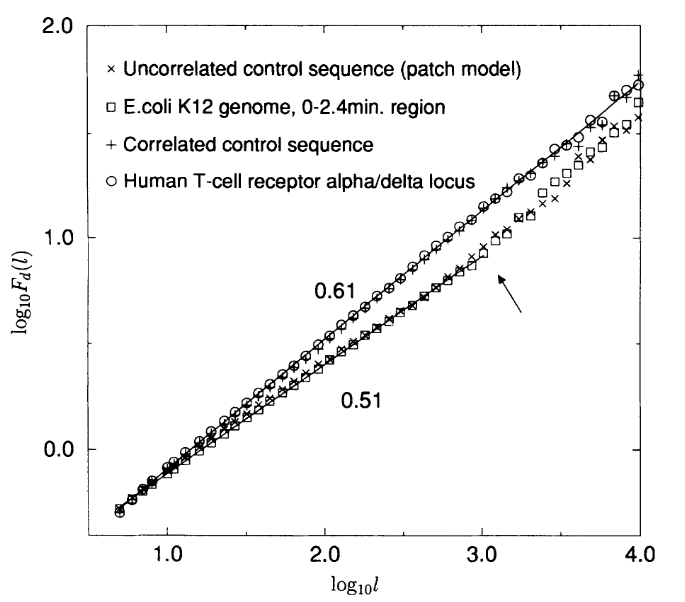
\includegraphics[width=.8\textwidth]{../Figures/peng.png}
	\\{\footnotesize Fonte: \cite{Peng1994}}
	\label{fig:peng01}
\end{figure}

Uma generalização multifractal do \dfa~foi proposta por \citeonline{kantelhardtMultifractalDetrendedUctuation2002}. Apresentado na Equação~\ref{eq:multifractal},onde o valor de $q$ representa a ordem da função \dfa~calculada. Quando $q=2$ a equação assume o valor do \dfa. No caso de $q=0$ a média exponencial é utilizada para a medição. Esses resultados também foram expandidos, baseando-se no \dcca~para a correlação multifractal entre séries temporais \cite{zhouMultifractalDetrendedCrosscorrelation2008}.

\begin{equation}\label{eq:multifractal}
  \begin{split}
  q \neq 0,
  \\[10pt]
  F_q(s) \equiv \left\{ \frac{1}{2N_s} \sum_{v=1}^{2N_s} \left[ F^2(v,s) \right]^{q/2} \right\}^{1/q},
  \\[10pt]
  q=0,
  \\[10pt]
  F_0(s) \equiv \exp\left\{ \frac{1}{4N_s} \sum_{v=1}^{2N_s} \ln\left[ F^2(v,s) \right] \right\} \sim s^{h(0)}
  \end{split}
  \end{equation}

\section{Variantes de correlação cruzada baseados no \dcca}
\label{ss:vari_cross}

Duas variantes do \dcca~que lidam com correlação cruzada já foram apresentados nesta pesquisa: O \pdcca~e o \dmc. Além desses métodos, este trabalho destaca mais alguns trabalhos: \textit{Multivariate Detrended Fluctuation Analysis}~($MVDFA$)~\cite{xiongDetrendedFluctuationAnalysis2017}, \textit{Generic Multichannel DFA}($GMDFA$)~\cite{naveedFullyMultivariateDetrended2025} e o \textit{Detrended Partial Cross-correlation Coefficient}~($DPCCA$)~\cite{yuanDetrendedPartialCrossCorrelationAnalysis2015}.

Diferente do \dmc, que estabelece um valor de função, onde a correlação é medida entre um conjunto de variáveis independentes e uma variável dependente, o $MVDFA$ calcula um valor único para qualquer combinação de séries temporais, representando uma generalização do DFA para múltiplas variáveis. Neste método, divide-se a série temporal em um conjunto de caixas não sobreposto, eventualmente perdendo alguns valores no final da série, mas repetindo o processo do fim para o começo da reta para compensar. Após a interpolação dos polinômios, a função local, em cada caixa e dada pela Equação~\ref{eq:mvdfa}, one a norma euclidiana~(Equação~\ref{eq:euclidean_norm}) é utilizada para o cálculo.


\begin{equation}\label{eq:mvdfa}
  F^2(v, s)=\frac{1}{s} \sum_{t=1}^s\left\|\left(Y_{l_v+t, 1}, Y_{l_v+t, 2}, \ldots, Y_{l_v+t, p}\right)-\left(\tilde{Y}_{\cdot, 1}, \tilde{Y}_{\cdot, 2}, \ldots, \tilde{Y}_{,, p}\right)\right\|^2
  \end{equation}

\begin{equation}\label{eq:euclidean_norm}
    \|X-Y\|=\left\|\left(x_1, x_2, \ldots, x_n\right)-\left(y_1, y_2, \ldots, y_n\right)\right\|=\sqrt{\sum_{i=1}^n\left(x_i-y_i\right)^2}
\end{equation}

Terminando o cálculo de forma semelhante ao apresentado no algoritmo do \dfa~, como mostrado na Equação~\ref{eq:mvdfa_end}. O $MGDFA$ substitui a norma euclideana pela norma de Mahalanobis. Estes métodos não possuem qualquer relação com o \dcca e, por extensão, com o \pdcca.

\begin{equation}\label{eq:mvdfa_end}
    F_{M V D F A}(s)=\left\{\frac{1}{2 N_s} \sum_{v=1}^{2 N_s}\left[F^2(v, s)\right]\right\}^{1 / n}
\end{equation}

Já o $DPDCCA$ aplica a mesma matriz utilizada no cálculo do \dmc, apresentado na Equação~\ref{eq:dmc}, cuja forma antes da inversão é apresentada na Equação~\ref{eq:p_dcca_matrix}. A matriz é denominada de $C(n)$~(Equação~\ref{eq:dpdcca_mat}). 


\begin{equation}\label{eq:dpdcca_mat}
  C(n)=\boldsymbol{\rho}^{-\mathbf{1}}(n)=\left(\begin{matrix}
  C_{1,1}(n) & C_{1,2}(n) & \ldots & 
  C_{1, m}(n) \\
  C_{2,1}(n) & C_{2,2}(n) & \ldots & C_{2, m}(n) \\
  \vdots & \vdots & & \vdots \\
  C_{m, 1}(n) & C_{m, 2}(n) & \ldots & C_{m, m}(n)
  \end{matrix}\right)
\end{equation}

O cálculo final do $DPDCCA$ é realizado pela Equação~\ref{eq:dpdcca}, a partir dos valores obtidos pela inversão da matriz do \pdcca.

\begin{equation}\label{eq:dpdcca}
  \rho_{D P C C A}\left(j_1, j_2 ; n\right)=\frac{-C_{j_1, j_2}(n)}{\sqrt{C_{j_1, j_1}(n) \cdot C_{j_2, j_2}(n)}}
\end{equation}

O resultado deve ser analisado como a correlação entre as duas variáveis, desconsiderando a atuação das outras variáveis cujos valores de \pdcca foram utilizados na montagem da matriz na Equação~\ref{eq:p_dcca_matrix}.

\section{Aplicações dos métodos}
\label{ss:aplica}